\documentclass[a4paper,12pt]{article}
% pdf-Metadaten
\pdfinfo{    
     /Title (PDF-Titel) 
     /Subject   (PDF-Thema)    
     /Author  (Vorname Nachname) 
     /Keywords   (Stichwort1,Stichwort2)      
} 
\usepackage[T1]{fontenc}
\usepackage[utf8]{inputenc}
\usepackage{lmodern}
% für Deutsche Begriffe und Silbentrennung
\usepackage[ngerman]{babel}
% required for equations
\usepackage{amsmath}
% required to include graphics
\usepackage{graphicx}
% Abkürzungsverzeichnis
\usepackage{acronym}
% Stichwortverzeichnis
\usepackage{makeidx}
\makeindex
% Works around a bug in LaTeX, which results in a wrong vertical position of the title
% http://tex.stackexchange.com/questions/49959/wrong-vertical-position-of-heading-created-by-printindex
\usepackage{idxlayout}
% Zeilenabstand 1,5 Zeilen
\usepackage{setspace}
\onehalfspacing
% BibLaTeX benutzen
\usepackage[backend=biber,citestyle=alphabetic,bibstyle=alphabetic]{biblatex}
\addbibresource{bib/Bibliographie.bib}
\DeclareLabelalphaTemplate{
  \labelelement{
    \field[final]{shorthand}
    \field{label}
    \field[strwidth=3,strside=left,ifnames=1]{labelname}
    \field[strwidth=1,strside=left]{labelname}
  }
\labelelement{
        \literal{-}
      }
  \labelelement{
    \field[strwidth=2,strside=right]{year}
  }
}
% Seitenränder anpassen
\usepackage{geometry}
\geometry{left=2cm, right=2cm, top=2.5cm, bottom=2cm}
% allows including eps graphics
\usepackage{epstopdf}
% makes TOC and references clickable
\usepackage[hidelinks]{hyperref}
\title{My first \LaTeX{} document}
\author{Jon Doe}

\begin{document}

\newpage\null\thispagestyle{empty}\newpage
\newpage
\pagestyle{empty}

\begin{figure}[t]
	\centering
	
\includegraphics[width=0.35\textwidth]{Bilder/Logo/logo-h-da.eps}
\end{figure}

\vfill

\begin{center}
\Large Hochschule Darmstadt \\
\normalsize \textsc{- Fachbereich Maschinenbau und Kunststofftechnik -} \\

\vfill

\Huge Der Titel der Arbeit \\
\normalsize
\vspace{12pt}
Abschlussarbeit zur Erlangung des akademischen Grades \\ 
Bachelor of Science (B.Sc.)

\vfill

vorgelegt von \\
Vorname Nachname

\vfill

\begin{tabular}[h]{p{4cm}l}
	Referent(in): & Name des Erstbetreuers\\
	Korreferent(in):  & Name des Zweitbetreuers \\
\end{tabular}

\end{center}

\newpage
\pagestyle{plain}
\section*{Eidesstattliche Erklärung}
\addcontentsline{toc}{section}{Eidesstattliche Erklärung}
Ich versichere hiermit, dass ich die vorliegende Arbeit selbständig verfasst und keine
anderen als die im Literaturverzeichnis angegebenen Quellen benutzt habe. \\

\noindent Alle Stellen, die wörtlich oder sinngemäß aus veröffentlichten oder noch nicht veröffentlichten Quellen entnommen sind, sind als solche kenntlich gemacht. \\

\noindent Die Zeichnungen oder Abbildungen in dieser Arbeit sind von mir selbst erstellt worden oder mit
einem entsprechenden Quellennachweis versehen. \\

\noindent Diese Arbeit ist in gleicher oder ähnlicher Form noch bei keiner anderen Prüfungsbehörde
eingereicht worden.
\newline\newline
Darmstadt, den \today
\newpage
\begin{abstract}
Weit hinten, hinter den Wortbergen, fern der Länder Vokalien und Konsonantien leben die Blindtexte. Abgeschieden wohnen sie in Buchstabhausen an der Küste des Semantik, eines großen Sprachozeans. Ein kleines Bächlein namens Duden fließt durch ihren Ort und versorgt sie mit den nötigen Regelialien. Es ist ein paradiesmatisches Land, in dem einem gebratene Satzteile in den Mund fliegen. Nicht einmal von der allmächtigen Interpunktion werden die Blindtexte beherrscht – ein geradezu unorthographisches Leben. Eines Tages aber beschloß eine kleine Zeile Blindtext, ihr Name war Lorem Ipsum, hinaus zu gehen in die weite Grammatik. Der große Oxmox riet ihr davon ab, da es dort wimmele von bösen Kommata, wilden Fragezeichen und hinterhältigen Semikoli, doch das Blindtextchen ließ sich nicht beirren. Es packte seine sieben Versalien, schob sich sein Initial in den Gürtel und machte sich auf den Weg. Als es die ersten Hügel des Kursivgebirges erklommen hatte, warf es einen letzten Blick zurück auf die Skyline seiner Heimatstadt Buchstabhausen, die Headline von Alphabetdorf und die Subline seiner eigenen Straße, der Zeilengasse. Wehmütig lief ihm eine rhetorische Frage über die Wange, dann setzte es seinen Weg fort.
\end{abstract}
\addcontentsline{toc}{section}{Zusammenfassung}
\newpage
\section*{Vorwort}
\addcontentsline{toc}{section}{Vorwort}
Eine wunderbare Heiterkeit hat meine ganze Seele eingenommen, gleich den süßen Frühlingsmorgen, die ich mit ganzem Herzen genieße. Ich bin allein und freue mich meines Lebens in dieser Gegend, die für solche Seelen geschaffen ist wie die meine. Ich bin so glücklich, mein Bester, so ganz in dem Gefühle von ruhigem Dasein versunken, daß meine Kunst darunter leidet. Ich könnte jetzt nicht zeichnen, nicht einen Strich, und bin nie ein größerer Maler gewesen als in diesen Augenblicken.

Wenn das liebe Tal um mich dampft, und die hohe Sonne an der Oberfläche der undurchdringlichen Finsternis meines Waldes ruht, und nur einzelne Strahlen sich in das innere Heiligtum stehlen, ich dann im hohen Grase am fallenden Bache liege, und näher an der Erde tausend mannigfaltige Gräschen mir merkwürdig werden; wenn ich das Wimmeln der kleinen Welt zwischen Halmen, die unzähligen, unergründlichen Gestalten der Würmchen, der Mückchen näher an meinem Herzen fühle, und fühle die Gegenwart des Allmächtigen, der uns nach seinem Bilde schuf, das Wehen des Alliebenden, der uns in ewiger Wonne schwebend trägt und erhält; mein Freund! Wenn's dann um meine Augen dämmert, und die Welt um mich her und der Himmel ganz in meiner Seele ruhn wie die Gestalt.
\newpage
\addcontentsline{toc}{section}{Inhaltsverzeichnis}
\tableofcontents
\newpage
% http://kleinmann.eit.h-da.de/99_ThesisInfos/

\section{Einführung / Problembeschreibung} 
Jemand "`musste"' Josef K. verleumdet haben, denn ohne dass er etwas Böses \cite{Pleisteiner.2007} getan hätte, wurde er eines Morgens verhaftet. »Wie ein Hund!« sagte er, es war, als sollte die Scham ihn überleben \ac{KDE} \cite[S.55ff]{Accardi.2010}. Als Gregor Sams eines Morgens aus unruhigen Träumen erwachte, fand er sich in seinem Bett zu einem ungeheuren Ungeziefer \index{Ungeziefer} verwandelt \cite{Lewis.2010}.
\subsection{Was ist die Motivation?}
\blindtext

\begin{figure}[h]
	\centering 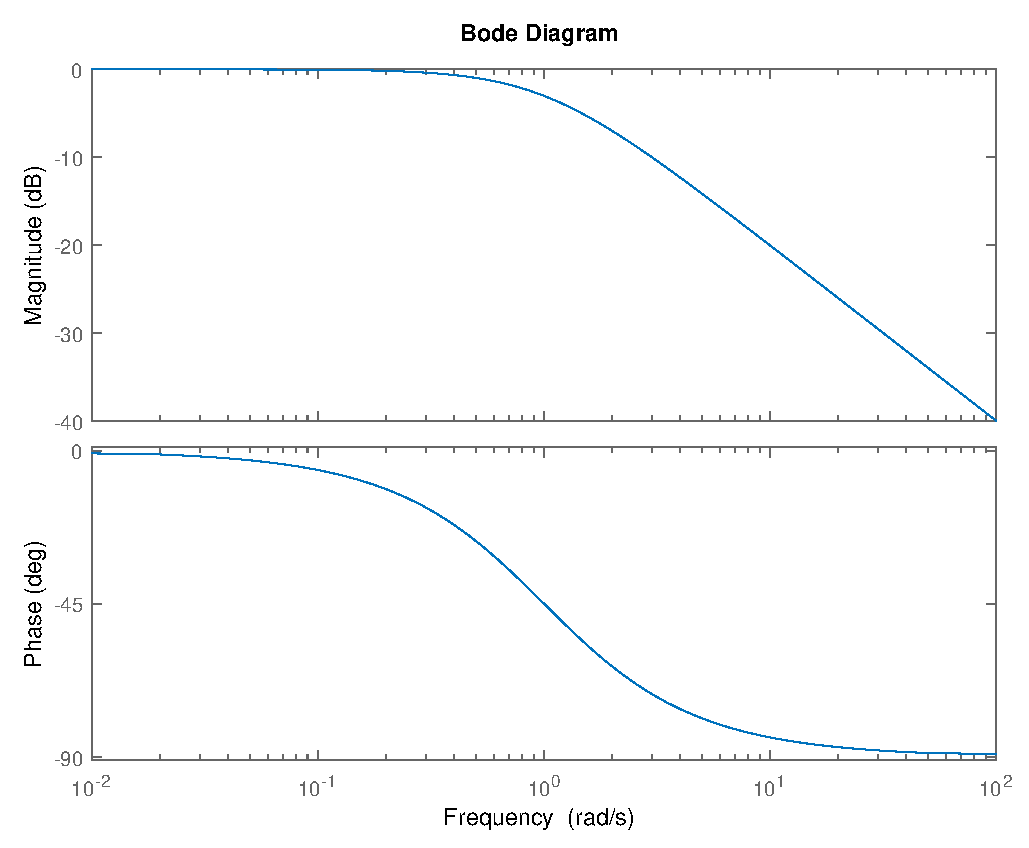
\includegraphics[width=0.5\textwidth]{fig/PT1/PT1.eps}
	\caption{Bodediagramm PT1}
\end{figure}

\blindtext

\begin{IEEEeqnarray}{rCl}
	a & = & b + c \\
	& = & d + e + f + g + h \\
	& = & p + q + r + s
\end{IEEEeqnarray}

\blindtext

\begin{table}[h]
	\centering
	\begin{tabular}[h]{|c|c|}
		\hline
		$U_e$ / V& $U_a$ / V\\ \hline
		0.1 & 0.2 \\ \hline
		0.2 & 0.4 \\ \hline
		0.3 & 0.6 \\ \hline
		0.4 & 0.8 \\ \hline
		0.5 & 1 \\ \hline
	\end{tabular}
	\caption{Messergebnisse}
\end{table}

\subsection{Was ist die Aufgabe?}
\blindtext
\subsection{Was ist das Ziel dieser Arbeit?}
\blindtext
\subsection{Was war der Status Quo, bevor mit dieser Arbeit begonnen wurde?}
\blindtext
\subsubsection{Firma X hat etwas in der Vergangenheit auf diesem oder jenem Wege gemacht…}
\blindtext
\section{Problemlösung}
\blindtext
\subsection{Was sind die Optionen / Welche prinzipiellen Lösungen sind möglich?}
\blindtext
\subsection{Stand der Technik / Wie wird es woanders gemacht?}
\blindtext
\subsection{Was ist der in dieser Arbeit gewählte Ansatz?}
\blindtext
\subsection{Weshalb wurde dieser Ansatz gewählt / Was unterscheidet ihn von anderen / Was ist neu / Was ist bekannt?}
\blindtext
\subsection{Detaillierte Beschreibung der Problemlösung}
\blindtext
\section{Implementierung und Test}
\blindtext
\subsection{Wie wurde es implementiert}
\blindtext
\subsection{Wie wurde getestet}
\blindtext
\subsection{Warum wurde so getestet?}
\blindtext
\section{Validierung}
\blindtext
\subsection{Was sind die Ergebnisse}
\blindtext
\subsection{Vor- und Nachteile des entwickelten Systems}
\blindtext
\section{Zusammenfassung / Fazit / zukünftige Arbeit}
\blindtext
\subsection{Was wurde getan}
\blindtext
\subsection{Was muss noch getan werden / Wie kann das System verbessert werden?}
\blindtext
\newpage
\addcontentsline{toc}{section}{Literatur}
\printbibliography
\newpage
\renewcommand{\indexname}{Stichwortverzeichnis}
\printindex
\addcontentsline{toc}{section}{Stichwortverzeichnis}
\newpage
\section*{Abkürzungsverzeichnis}
\addcontentsline{toc}{section}{Abkürzungsverzeichnis}
\begin{acronym}[Bash]
 \acro{KDE}{K Desktop Environment}
 \acro{SQL}{Structured Query Language}
 \acro{Bash}{Bourne-again shell}
 \acro{JDK}{Java Development Kit}
 \acro{VM}{Virtuelle Maschine}
 \acro{I2C}[IC]{Inter-Integrated Circuit}
\end{acronym}
\newpage
\addcontentsline{toc}{section}{Abbildungsverzeichnis}
\listoffigures
\newpage
\addcontentsline{toc}{section}{Tabellenverzeichnis}
\listoftables
\newpage
\section*{Anhang}
\addcontentsline{toc}{section}{Anhang}
\end{document}